% !TEX root = ../main.tex

\chapter{基于有监督预训练的蛋白质表征学习}

在过去的几十年里,蛋白质序列数据的快速增长为推断蛋白质的理化性质和功能提供了巨大的机会。 许多机器学习方法已成功应用于基于氨基酸序列信息的各种蛋白质分类任务,然而模型性能往往受到数据库中标记数据不足的影响。受到自然语言处理中预训练策略的启发,通过语言建模的无监督预训练已被引入生物序列分析从而缓解小数据问题。然而,这些无监督的预训练方法通常是计算密集型的,进行预训练需要消耗大量的计算资源,成本很高。

本章中,我们提出了一个用于进行蛋白质序列表征学习的预训练平台。研究的关键在于如何有效的利用蛋白质信息,尽可能地挖掘蛋白质中氨基酸表示的信息,通过预训练模型有效的处理氨基酸特征并对其进行表征学习。为了验证蛋白质序列的特征表示结果,我们开发的模型选取蛋白质研究中最典型的蛋白质分类问题对其进行研究,在三个蛋白质分类下游任务中(包括III 型分泌效应蛋白(T3SE)的识别、亚细胞定位的预测和信号肽的识别)进行实验。

本章将详细的介绍我们提出的 ProtPlat 模型,该模型完成了有监督的预训练氨基酸嵌入表征,进一步可以将预训练模型应用于各种蛋白质分类任务,同时我们实现了一个 Web 服务,用户可以下载经过预训练的词嵌入表征向量,并且通过提交自己的训练集和预测集获得蛋白质分类的预测类别。本章主要分为四个部分展开:分别是实验数据集构建、数据处理、基于蛋白质预训练表征学习的模型以及实验结果。

\section{实验数据集构建}
我们首先在 Pfam 数据库上对蛋白质序列进行大规模有监督的预训练表征学习,从而获得一个良好的氨基酸词嵌入表征。接着我们利用下游任务数据集对预训练的嵌入表征进行微调,使得他们在不同的下游任务上都有更好的表现。

\subsection{蛋白质表征学习预训练数据集} \label{4.1.1}
由于预训练需要大规模的语料库,因此我们使用 Pfam 数据库 \cite{finn2010pfam}。Pfam 是一个被广泛使用蛋白质家族结构域数据库,它是一系列蛋白质家族的集合,依赖多序列比对和隐马尔可夫模型(HMM)鉴定一个或者多个蛋白质的功能结构域,根据序列和结构的相似性将蛋白质序列划分为不同的家族,数据库中包括超过 3400 万个蛋白质序列。我们使用 Pfam 数据库中的 family 标签作为是预训练的目标,整个有监督预训练的过程是一个多分类问题。

由于 Pfam 数据中库蛋白质的 family 标签过多(2019 年发布的 32.0 版本中有 17929 个不同的 family 标签),为了避免数据分布极度不平衡导致的问题(如表 \ref{table:4.1.1}所示),我们去除了样本数小于500的蛋白质家族,总共得到了 7249 个蛋白质家族和 32853084 条蛋白质序列。

\begin{table}[!htbp]
\centering
\bicaption[Pfam 数据库中包含不同序列数的蛋白质家族数]{Pfam 数据库中包含不同序列数的蛋白质家族数。}{Numbers of protein families with different numbers of sequences in Pfam.}
\scalebox{1.3}{
\begin{tabular}{c|c}
\toprule
\# 蛋白质序列 & \# 蛋白质家族 \\
\midrule
$<$100 & 5474 \\ 
\hline
$<$200 & 7433 \\
\hline
$<$300 & 8775 \\
\hline
$<$500 & 10523 \\ 
\hline
$\geq$500 & 7249 \\
\bottomrule
\end{tabular}}
\label{table:4.1.1}
\end{table}


\subsection{下游蛋白质分类任务数据集}
为了评估经过预训练得到的词嵌入表征向量的性能,我们试验了三个下游蛋白质分类任务,如下所述。

\subsubsection{任务I:III 型分泌效应蛋白(T3SE)的识别}

III型分泌系统(TTSS)与许多革兰氏阴性病原体毒力因子的分泌有关。III 型分泌系统的效应蛋白(T3SE)直接从细菌细胞分泌到宿主细胞中,然后在疾病进展和免疫反应抑制中发挥作用。识别 III 型分泌效应蛋白有助于揭示 TTSS 的机制。然而,由于缺乏保留膜体或者分泌信号,T3SEs 的预测是一项特别具有挑战性的工作,现有方法主要是利用氨基酸序列的统计特征。这里,我们采用与 WEDeepT3 \cite{fu2019wedeept3} 相同的数据集 BEAN 2.0 \cite{dong2015bean},这是目前识别 T3SE 任务最大的数据集,其使用 CD-hit 工具 \cite{li2006cd} 去除蛋白质序列的冗余,并将序列一致性参数设置为 40\%。该数据集中一共包括 525 个训练样本(241 个 T3SE 和 284 个非 T3SE)和 138 个测试样本(46 个 T3SE 和 92 个非 T3SE)。 数据统计见表 \ref{table:4.1.2-1}。

\begin{table}[!htbp]
\centering
\bicaption[识别III型分泌效应蛋白数据集]{识别III型分泌效应蛋白数据集。}{Dataset of type III secreted effectors.}
\scalebox{1.3}{ 
\begin{tabular}{ c | c |c |c} 
 \toprule
  数据集 & T3SE & non-T3SE &总数\\  
 \midrule
 训练集 \#& 241 & 284 &525\\ 
 \hline
 测试集 \#& 46 & 92 &138\\ 
 \bottomrule
 \end{tabular}}
\label{table:4.1.2-1}
\end{table}

\subsubsection{任务II:预测蛋白质亚细胞定位}

蛋白质在细胞中的位置与其功能密切相关。只有在合适的亚细胞位置,蛋白质才能正确发挥其功能。细胞中蛋白质定位的计算预测一直是生物信息学领域的热门话题,目前大多数现有预测工具都是基于蛋白质序列和机器学习方法 \cite{cheng2018ploc, nair2005mimicking, 2010YLoc}。 我们使用经典的亚细胞定位基准集 BaCeILo \cite{pierleoni2006bacello},包括来自动物(Animals)、真菌(Fungi)和植物(Plants)的蛋白质序列,位于四个亚细胞区室,分别是细胞核、细胞质、线粒体和分泌途径。BaCeILo 的数据统计见表 \ref{table:4.1.2-2}。
% 此外,我们还使用了 DeepLoc[4]中使用的最新数据集,包括位于10个亚细胞区室的13858个蛋白质序列,分别是细胞核、细胞质、细胞外、线粒体、膜体、内质网、质体、高尔基体、溶酶体和过氧化物酶体。

\begin{table}[!htbp]
\centering
\bicaption[蛋白质亚细胞定位数据集]{蛋白质亚细胞定位数据集。}{Datasets of protein subcellular localization.}
\scalebox{1.3}{
 \begin{tabular}{ c | c | c | c | c | c} 
 \toprule
 数据集 & cy & mi & nu & sp & 总数 \\
 \midrule
 Animals 训练集 \# & 302 & 153 & 803 & 632 & 1890 \\ 
 \hline
 Animals 测试集 \#& 137 & 35 & 363 & 172 & 707 \\
 \hline
 Fungi 训练集 \#& 181 & 177 & 589 & 72 & 1019 \\
 \hline
 Fungi 测试集 \#& 30 & 11 & 122 & 16 & 179 \\
 \hline
 Plants 训练集 \#& 52 & 57 & 60 & 35 & 204 \\
 \hline
 Plants 测试集 \#& 6 & 10 & 61 & 6 & 83 \\
 \bottomrule
 \end{tabular}}
\begin{tablenotes}\scriptsize
\item [a] $^*$其中cy代表细胞核,mi代表细胞质,nu代表线粒体,sp代表分泌途径\\
\end{tablenotes}
 \label{table:4.1.2-2}
\end{table}

\subsubsection{任务III:信号肽的识别}
信号肽通常位于蛋白质序列末端,长度一般为 5 - 30 个氨基酸。信号肽的主要功能是促进蛋白质在细胞外分泌或定位于某些细胞器,因此信号肽的鉴定可以为揭示蛋白质功能提供线索。我们考虑了两种类型的信号肽,分别是由 SPase I (Sec/SPI) 切割的 Sec 底物和其他底物。我们使用 SignalP 5.0 \cite{armenteros2019signalp} 中提供的信号肽数据集,其中蛋白质来自真核生物(Archaea)、古细菌(Eukaryotes)、革兰氏阳性菌(Gram-positive)和革兰氏阴性菌(Gram-negative)。SignalP 5.0 数据集的数据统计见表 \ref{table:4.1.2-3}。

\begin{table}[!htbp]
\centering
\bicaption[信号肽的识别数据集]{信号肽的识别数据集。}{Datasets of signal peptides.}
\scalebox{1.3}{
 \begin{tabular}{c | c | c | c} 
 \toprule
 数据集 & Sec/SPI & 其他 & 总数 \\
 \midrule
 Archaea 训练集 \# & 10 & 45 & 55 \\ 
  \hline
 Archaea 测试集 \#& 50 & 132 & 182 \\
  \hline
 Eukaryotes 训练集 \#& 2404 & 7409 & 9813 \\
  \hline
 Eukaryotes 测试集 \#& 210 & 7247 & 7457 \\
  \hline
 Gram-negative 训练集 \#& 419 & 1126 & 1545 \\
  \hline
 Gram-negative 测试集 \#& 90 & 693 & 783 \\
  \hline
 Gram-positive 训练集 \#& 164 & 370 & 534 \\
  \hline
 Gram-negative 测试集 \#& 25 & 364 & 389 \\ 
 \bottomrule
 \end{tabular}}
 \label{table:4.1.2-3}
\end{table}


\section{数据处理}
\subsection{输入蛋白质序列的处理}
在蛋白质有监督的预训练任务和蛋白质分类任务中,输入的都是蛋白质序列。蛋白质序列是由20几种氨基酸排列组合形成的一串连续序列,因此在蛋白质序列中没有一个特定的划分边界,需要我们利用不同的序列切割方法进行词划分的尝试,然后利用深度学习网络在分词中提取特征表示信息。针对输入的蛋白质序列处理的关键首先在于对蛋白质序列进行切分,获取对应的词汇表。

和自然语言处理中的文本序列不同的是,蛋白质序列中没有已知的具有语义的单词作为划分边界,因此我们无法通过生物信息的意义判断合理的和不合理的分词。同时某个单词出现的频率和其表达的生物含义也无法意义对应。因此通常的做法是将蛋白质序列划分固定长度的短肽片段(即 k-mers,k 个氨基酸为一个单词)从而对词向量进行嵌入表征学习,应用到下游任务中。下面我们讨论了两种常用的蛋白质序列分割方法。

\subsubsection{不重叠的 $k-mer$ 切割方式}
在生物信息学领域,生物序列通常被分割成固定长度的 $k-mers$ 进行特征提取 \cite{asgari2015continuous, ofer2021language, yang2018learned, liu2019bioseq}。对于蛋白质序列来说,将连续的 $k$ 个氨基酸作为一个蛋白质的单词,接着对于剩余的蛋白质序列依次进行切分。通常,$k$ 的取值小于或等于 5,并且不能太大,因为随着 $k$ 的增加,$k-mer$ 词汇表空间将呈指数增长,这将导致极高的维度和单词频率的显著降低。最常见的不重叠 k-mer 切割方式是当 $k$ 的值为 1 时,此时每一个氨基酸表示一个单独的分词,此时蛋白质序列词汇表的大小为氨基酸的种类数。

不重叠的 $k-mer$ 切割方法的优点是简单方便。每个 $k-mer$ 不仅包含了单个氨基酸的信息,还包含其相邻 氨基酸的信息。但是,该分割方法的缺点也很明显。由于切分过于简单粗暴,直接将序列划分为 $k$ 个氨基酸组成的单词,导致将损失一部分的序列信息。另外,该切割方法只考虑固定长度的 $k-mer$ 分词。为了缓解这种限制,这里我们考虑包含所有长度小于或等于 k 的分词作为蛋白质序列的词汇表空间。以蛋白质序列 “MASPAAERKS” 为例,当k设置为3时,该序列的词汇表空间为
\{M, A, S, P, E, R, K, MA, SP, AA, ER, KS , MAS, PAA, ERK\} ,大小为 15。

\subsubsection{重叠的 $k-mer$ 切割方式}
使用不重叠 $k-mer$ 切割,切分起始位置的一点点偏移可能产生非常不同的切分词汇表。由于蛋白质序列的长度具有极大的不确定性,对于长度较短的蛋白质序列来说,对于切割起始位置的不同尤为敏感。为了避免这种由于单词划分带来的不确定性,重叠的 $k-mer$ 分割方法被广泛使用。该方法采用一个固定长度为 $k$ 的滑动窗口每次以步长为1的速度对蛋白质序列进行切割,在滑动窗口内的氨基酸作为一个蛋白质的单词,这样就考虑了序列中所有长度为 $k$ 的子串,比不重叠 $k-mer$ 的分割具有更大的特征空间。仍然以蛋白质序列 “MASPAAERKS” 为例,当k设置为3时,该序列的词汇表空间变为 \{M, A, S, P, E, R, K, MA, AS, SP, PA, AA, AE, ER, RK, KS, MAS, ASP, SPA, PAA, AAE, AER, ERK, RKS\},大小为24。可以看到, 重叠的 $k-mer$ 切割方式比不重叠的 $k-mer$ 切割方式可以保留更多的序列信息。和不重叠的 $k-mer$ 切割方式处理一样,我们考虑包含所有长度小于或等于 $k$ 的分词作为蛋白质序列的词汇表空间。

为了充分利用蛋白质序列的信息,我们接下来采用了重叠的 $k-mer$ 切割方式对蛋白质序列进行有监督的预训练,同时在蛋白质分类任务上进行验证。我们比较了使用这两种分割方法的模型性能,结果在第 4.4.1 节中讨论。

\subsection{预训练的数据处理}
在第 \ref{4.1.1} 节中提到,我们使用大型语料库 Pfam 数据库来执行有监督的预训练。Pfam 数据库的构建包括以下步骤(如图\ref{fig:data-process}所示):
\begin{itemize}
    \item [1)] 
    在 2019 年发布的 32.0 版本的 Pfam 数据库中下载了总共包含 17,772 个蛋白质家族和 34,353,433 条蛋白质序列; 
    \item [2)]
    提取每个蛋白质的家族(family)标签和蛋白质序列;
    \item [3)]
    通过删除少于 500 个样本的蛋白质家族,构建得到包含 7249 个蛋白质家族和 32,853,084 个序列的数据集。
  \end{itemize}

\begin{figure}[!htp] 
\centering
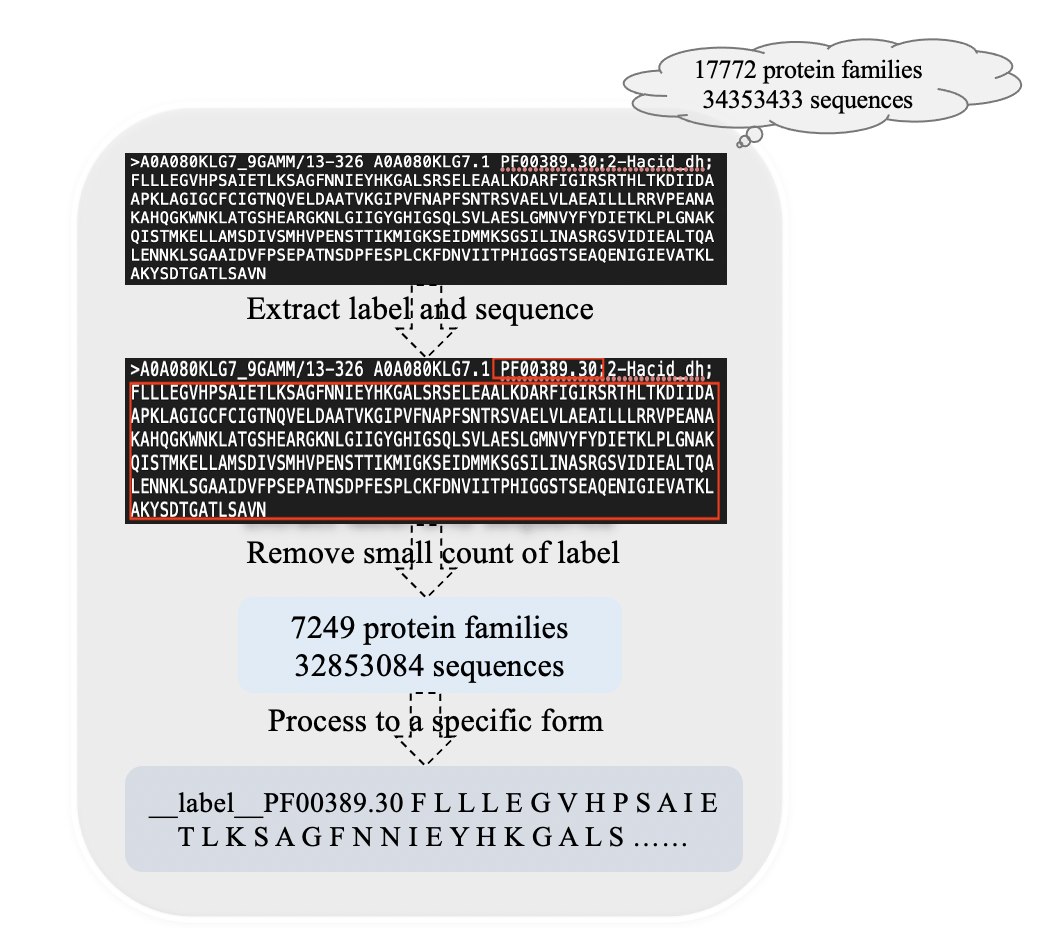
\includegraphics[width=0.95\textwidth]  {imgs/data-process.png}
\bicaption[Pfam 数据库的数据收集和过滤过程]
        {Pfam 数据库的数据收集和过滤过程。}
        {The data collection and filtering process of the Pfam database.}
\label{fig:data-process}
\end{figure}

\section{基于蛋白质预训练表征学习的模型}
\subsection{ProtPlat 模型}
为了描述 ProtPlat 模型的工作原理,我们定义了以下符号。

\begin{itemize}
    \item $C$:初始特征嵌入空间的大小,即用于分类任务的 k-mers (小于等于 k 的分词)的数量;
    \item $m$:嵌入表征向量的维度;
    \item $p$:隐藏层表征向量的维度;
    \item $n$:分类任务的标签数量;
    \item $V \in \mathbb{R}^{p*m}$:输入权重矩阵;
    \item $U \in \mathbb{R}^{n*p}$:输出权重矩阵
\end{itemize}

ProtPlat 模型的工作流程可以表述如下:
将 $(x^{(1)}, x^{(2)}, ..., x^{(C)}) \in \mathbb{R}^{m}$ 作为初始特征嵌入表征向量,通过一个全连接层获得嵌入表征向量,

\begin{equation}
    (h_1 = V \times x^{(1)}, h_2 = V \times x^{(2)},...,h_C = V \times x^{(C)}) \in \mathbb {R}^{p}.
\end{equation}

然后对所有的嵌入表征向量进行平均操作,得到平均嵌入表征向量,$\hat{h} \in \mathbb{R}^{p}$

\begin{equation}
    \hat{h} = \frac{\sum_{i\in \{1,2,\cdots, C\}} h_i}{C}. 
\end{equation}

接着将平均嵌入表征向量通过一个全连接层生成得分表示向量,$z \in \mathbb{R}^{n} $

\begin{equation}
    z = U \times \hat{h}.
\end{equation}

将得分表示向量通过层次 softmax 层转化为分类标签的概率分布,

\begin{equation}
    \hat{y} = softmax(z).
\end{equation}

ProtPlat 模型的主要结构是一个三层神经网络,如图 \ref{fig:protplat} 所示。模型的输入是一个 $C \times m$ 维矩阵,由蛋白质中长度小于或等于 $k$ 的分词的向量组成一个序列。例如,当 $k$ 设置为 3 时,输入涵盖所有的氨基酸、2-mer 和 3-mer 特征。其中每一个 $k-mer$ 的初始特征向量是它所包含的 $k$ 个氨基酸初始特征嵌入表示向量的平均值。

序列分类模型中的一个重要机制是层次 softmax 函数,它使用二叉树来表示所有类别。树中的每个叶子节点都表示一个类别,使得在具有大量标签的分类任务中有较高的学习效率。基于霍夫曼编码 \cite{han2015deep} 构建层次 softmax,对类别标签进行编码,可以大大减少模型的预测目标数量。模型中蛋白质序列的平均嵌入表示是一个隐藏变量,可以重复使用。这种架构类似于 CBow 模型 \cite{mikolov2013distributed},不同之处在于 ProtPlat 模型中的中心词被替换为序列标签。


\begin{figure}[!htp] 
\centering
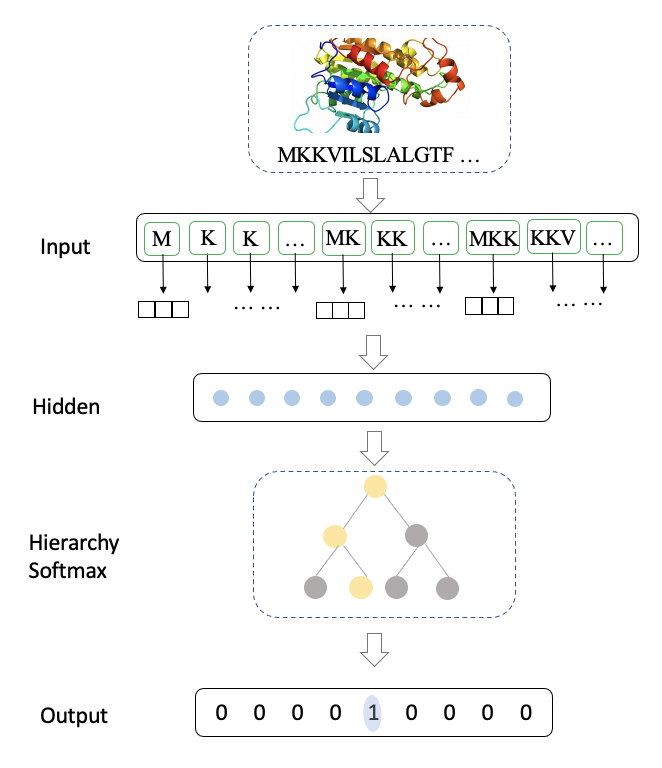
\includegraphics[width=0.85\textwidth]  {imgs/protplat.png}
\bicaption[ProtPlat 的模型架构]
        {ProtPlat 的模型架构。 $k-mer$ 嵌入表征向量送入神经网络并由隐藏层学习。输出类别标签由层次 Softmax 函数产生。}
        {Model architecture of ProtPlat. The k-mer embeddings are fed into the neural network and learned by the hidden layers. The output label is yielded by a hierarchy Softmax function. }
\label{fig:protplat}
\end{figure}

\subsection{两阶段训练过程}
为了将 ProtPlat 应用于下游任务,我们执行了一个两阶段的训练过程。

i) 预训练

我们使用 Pfam 数据库中的蛋白质序列和家族标签进行有监督的预训练,训练 ProtPlat 模型。 单个氨基酸的输入初始特征嵌入表示向量是随机初始化的,$k-mer$ 的初始特征嵌入表示向量是它所包含的 $k$ 个氨基酸初始特征嵌入表示向量的平均值。模型的输出是 Pfam 数据库中蛋白质序列所属的蛋白质家族标签。训练后,我们将每个氨基酸的嵌入表征向量保存为其经过预训练的特征嵌入表示向量,用于作为下游任务的输入初始特征嵌入表示向量(即 $x^{(i)}$)。

ii) 微调

微调阶段的训练过程与预训练几乎相同。不同之处在于输入和输出,其中氨基酸的输入是经过预训练的特征嵌入表示向量,$k-mer$ 的输入是它所包含的 $k$ 个氨基酸的经过预训练的特征嵌入表示向量的平均值,输出为下游分类任务的标签。

\section{实验结果}
\subsection{实验设置及评估指标}
对于预训练和微调过程,我们均随机抽取 20\% 的训练数据形成验证集。我们根据验证集上的模型性能选择最佳的超参数。表 \ref{table:4.4.1} 显示了 ProtPlat 中预训练阶段的超参数设置。值得注意的是,$k$ 的值是在预训练阶段确定的,在下游任务中保持不变。 对于每个下游任务,我们在其验证集上调整 epoch 和 learning rate。

\begin{table}[!htbp]
\centering
\bicaption[ProtPlat 中预训练阶段的超参数设置]{ProtPlat 中预训练阶段的超参数设置。}{Hyperparameter settings for pre-training in ProtPlat.}
\scalebox{1.3}{
\begin{tabular}{c|c}
\toprule
超参数 & 对应的值 \\
\midrule
k & 3 \\ 
\hline
epoch & 70 \\
\hline
learning rate & 0.15 \\
\hline
嵌入表征向量的维度 & 100 \\ 
\hline
隐藏层表征向量的维度 & 100 \\
\bottomrule
\end{tabular}}
\label{table:4.4.1}
\end{table}

为了评估 ProtPlat 模型的性能,我们在二元分类下游任务中使用了四个评估指标,包括准确率 (ACC)、$F_1$ 值 (F1 score)、presion (Pre) 和 recall (Rec)。它们的计算公式如公式(\ref{Eq:4-5})- 公式(\ref{Eq:4-8}) 所示。

\begin{equation}
    ACC = \frac{TP + TN}{TP + TN + FP + FN}
\label{Eq:4-5}
\end{equation}

\begin{equation}
    F_1 = \frac{2 * TP}{2 * TP + FP + FN}
\label{Eq:4-6}
\end{equation}

\begin{equation}
    Pre = \frac{TP}{TP + FP}
\label{Eq:4-7}
\end{equation}

\begin{equation}
    Rec = \frac{TP}{TP + FN}
\label{Eq:4-8}
\end{equation}
其中 $TP$、$TN$、$FP$ 和 $FN$ 分别表示真阳性、真阴性、假阳性和假阴性的数量。 

对于多分类问题,$F_1$ 值定义如公式(\ref{Eq:4-9})— 公式(\ref{Eq:4-11})所示:

\begin{equation}
    Pre = \frac{\sum TP_i}{\sum TP_i + \sum FP_i}
\label{Eq:4-9}
\end{equation}

\begin{equation}
    Rec = \frac{\sum TP_i}{\sum TP_i + \sum FN_i}
\label{Eq:4-10}
\end{equation}

\begin{equation}
    F_1 = \frac{2 * Pre * Rec}{Pre + Rec}
\label{Eq:4-11}
\end{equation}
其中,$i$ 代表多分类问题的类别索引,$TP_i$、$FP_i$ 和 $FN_i$ 分别表示第 i 个类别真阳性、假阳性和假阴性的数量。


\subsection{预训练表征学习的结果}
在这里,我们比较了经过预训练和没有经过预训练的 ProtPlat 模型的结果。经过预训练的 ProtPlat 模型使用预训练的嵌入表征向量作为每一个氨基酸的初始输入特征表示,而没有经过预训练的 ProtPlat 模型使用 one-hot 编码向量作为初始输入并随机初始化输入权重。

我们比较了它们在八个下游任务数据集上的性能,包括 T3SE 数据集、三个亚细胞定位数据集(来自 BaCeILo \cite{pierleoni2006bacello} 的植物、真菌和动物数据集)和四个信号肽数据集(来自 SignalP 5.0 \cite{armenteros2019signalp} 的古细菌、真核生物、革兰氏阳性和革兰氏阴性数据集)。结果如图 \ref{fig:pre-unpre} 所示。可以看出,预训练过程可以提高所有这些数据集的预测精度。$F_1$ 值增加了 0.03 — 0.08。此外,我们对性能差异进行了统计显着性分析。对于下游任务的每个数据集,我们分别在预训练和没有经过预训练的情况下运行 ProtPlat 模型 30 次,成对 $t$ 检验的 $p-value$ 值展示在表 \ref{table:4.4.2-1} 和 表 \ref{table:4.4.2-2} 中。对于所有的下游任务而言,$p-values$ 值都远小于 0.01,表明经过预训练的 ProtPlat 模型明显优于没有预训练的模型。

\begin{figure}[!htp] 
\centering
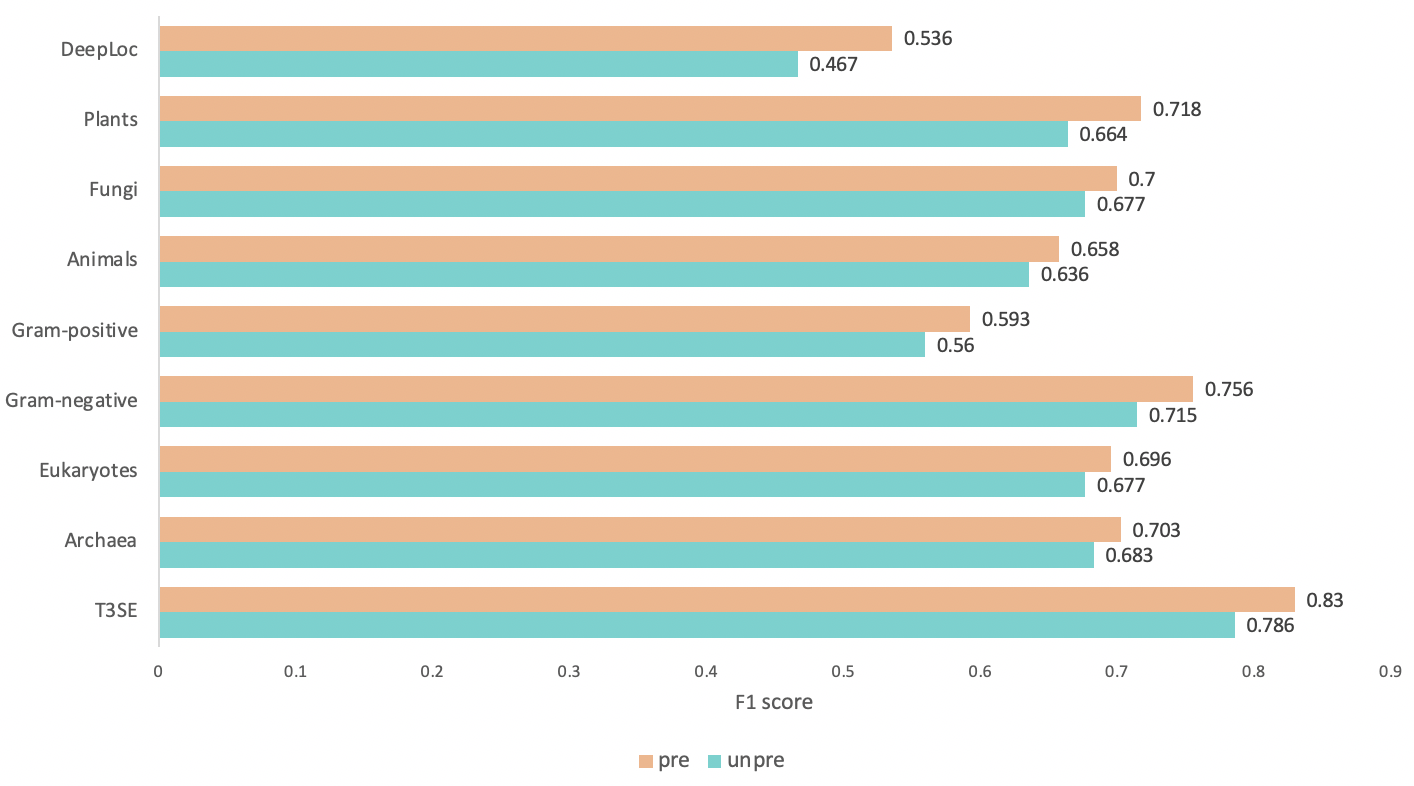
\includegraphics[width=1\textwidth]  {imgs/pre-unpre.png}
\bicaption[ProtPlat 有无经过预训练的 $F_1$ 值对比]
        {ProtPlat 有无经过预训练的 $F_1$ 值对比。}
        {F1 score comparison between models with and without pre-training. }
\label{fig:pre-unpre}
\end{figure}


\begin{table}[!htbp]
\centering
\bicaption[经过(w)和不经过(w/o)预训练的 Protplat 模型 ACC 的显着性分析]{经过(w)和不经过(w/o)预训练的 Protplat 模型 ACC 的显着性分析。}{Significance analysis of accuracy for models with (w) and without (w/o) pre-training.}
\begin{tabular}{c|c|c|c|c|c}
\toprule
\multirow{2}*{数据集} & \multicolumn{2}{c|}{平均值} & \multicolumn{2}{c|}{方差} & \multirow{2}*{p-value} \\
\cline{2-5}
&$w/o\quad pre$&$w\quad pre$&$w/o\quad pre$&$w\quad pre$ &   \\
\midrule
T3SE&0.786&0.830& 4.29E-05&3.34E-05& 6.39E-12\\
\hline
Animals&0.636&0.658&0.05E-05&1.68E-05 & 1.07E-08\\ 
\hline
Fungi&0.677&0.700& 3.41E-05&6.37E-05 &9.53E-07\\
\hline
Plants&0.664&0.718&3.79E-05&5.47E-05 &8.25E-13\\
\hline
Archaea&0.765&0.790& 5.13E-05&3.24E-05& 3.65E-07\\
\hline
Eukaryotes&0.923&0.947&3.21E-05&1.58E-05& 9.13E-09\\
\hline
Gram-negative&0.715&0.751&4.97E-05&8.62E-06&3.69E-10\\
\hline
Gram-positive&0.784&0.810& 3.47E-05&6.53E-05& 3.68E-09\\
\bottomrule
\end{tabular}
\label{table:4.4.2-1}
\end{table}

\begin{table}[!htbp]
\centering
\bicaption[经过(w)和不经过(w/o)预训练的 Protplat 模型 $F_1$ 值的显着性分析]{经过(w)和不经过(w/o)预训练的 Protplat 模型 $F_1$ 值的显着性分析。}{Significance analysis of F1 score for models with (w) and without (w/o) pre-training.}
\begin{tabular}{c|c|c|c|c|c}
\toprule
\multirow{2}*{数据集} & \multicolumn{2}{c|}{平均值} & \multicolumn{2}{c|}{方差} & \multirow{2}*{p-value} \\
\cline{2-5}
&$w/o\quad pre$&$w\quad pre$&$w/o\quad pre$&$w\quad pre$ &   \\
\midrule
T3SE&0.786&0.830& 4.29E-05&3.34E-05& 6.39E-12\\
\hline
Animals&0.636&0.658&0.05E-05&1.68E-05 & 1.07E-08\\ 
\hline
Fungi&0.677&0.700& 3.41E-05&6.37E-05 &9.53E-07\\
\hline
Plants&0.664&0.718&3.79E-05&5.47E-05 &8.25E-13\\
\hline
Archaea&0.683&0.703& 8.47E-05&4.27E-05& 2.56E-05\\
\hline
Eukaryotes&0.677&0.696&1.71E-05&2.01E-05& 1.68E-08\\
\hline
Gram-negative&0.715&0.756&1.39E-05&2.42E-05&4.50E-14\\
\hline
Gram-positive&0.56&0.593& 4.31E-05&5.32E-05& 3.61E-09\\
\bottomrule
\end{tabular}
\label{table:4.4.2-2}
\end{table}

\subsection{ProtPlat 与现有方法在下游任务上的比较}
\subsubsection{任务I:III 型分泌效应蛋白(T3SE)的识别}

III 型分泌效应子的识别是一个二元分类问题,即 T3SE 和非 T3SE。 为了评估 ProtPlat 模型的性能,我们将其与现有的代表性方法进行比较,包括 WEDeepT3 \cite{fu2019wedeept3}、BPBAac \cite{wang2011high}、EffectiveT3 \cite{arnold2009sequence}、T3\_MM \cite{wang2013t3_mm}、DeepT3 \cite{xue2019deept3}、Bastion3 \cite{wang2019bastion3} 和 BEAN 2.0 \cite{dong2015bean}。 

ProtPlat 模型在 WEDeepT3 的测试集上得到的结果如表\ref{table:4.4.3-1}所示。可以看出,ProtPlat取得了最好的性能。 与第二好的模型 WEDeepT3 相比,经过预训练的 ProtPlat 模型的 $F_1$ 值提高了 0.128,准确率提高了 0.021,这印证了预训练嵌入表征学习的分类性能。

\begin{table}[!htbp]
\centering
\bicaption[预测 III 型分泌效应蛋白的模型性能比较]{预测 III 型分泌效应蛋白的模型性能比较。}{Performance comparison for the prediction of type III secreted effectors.}
\scalebox{1.2}{
 \begin{tabular}{c | c | c } 
    \toprule
模型 & ACC & $F_1$ \\
 \midrule
WEDeepT3 & 0.812 & 0.705 \\ 
 \hline
BPBAac &0.609 &0.339\\
 \hline
EffectiveT3 &0.696 &0.512\\
 \hline
T3\_MM & 0.718 &0.581\\
 \hline
DeepT3 &0.594 &0.486\\
 \hline
Bastion3 &0.739 &0.673\\
 \hline
BEAN 2.0&0.761 &0.692\\
 \hline
ProtPlat & \textbf{0.833} & \textbf{0.833} \\ 
 \bottomrule
 \end{tabular}}
 \label{table:4.4.3-1}
\end{table}
其中,基线方法的准确率和 $F_1$ 值是从 WEDeepT3 \cite{fu2019wedeept3} 中提取的。所有方法都在相同的测试集上进行评估。


\subsubsection{任务II:预测蛋白质亚细胞定位}
对于蛋白质亚细胞定位,我们使用 BaCeILo \cite{pierleoni2006bacello} 中的数据集,并且与 Euk-mPLoc \cite{cheng2018ploc}、LOCTree \cite{nair2005mimicking}、BaCeILo \cite{pierleoni2006bacello}、 YLoc \cite{2010YLoc} 等基线方法进行比较。通过准确率(ACC)和 $F_1$ 值来评估模型的分类预测性能。对于所有的三个数据集植物(Plants)、真菌(Fungi)和动物(Animals),ProtPlat 都实现了具有竞争力的模型性能。尤其是在真菌(Fungi)数据集上,ProtPlat 明显优于其他模型($F_1$ 值和准确率(ACC)都提高了 10\% 以上),如表\ref{table:4.4.3-2}所示,这表明小数据集可能会从预训练中受益更多。对于小数据集本身来说标签数据量较少,提供的蛋白质领域信息较少,通过大数据量的预训练嵌入表征学习,可以为小数据集提供较为丰富的先验知识,解决了小数据集上蛋白质预测性能较低的问题。

基线模型的训练集不同 \cite{2010YLoc},并且很多基线模型都是更通用的预测器,可以预测 4 个以上的亚细胞位置,比如 YLoc-HighRes、YLoc+、MultiLoc2-HighRes、WoLF PSORT、Euk- mPLoc 和 LOCTree,因此它们的性能可能比专门为这四个位置训练的预测器差。值得注意的是,几乎所有的基线方法都利用了多个来源的信息作为输入特征,包括某些领域知识,例如蛋白质功能域和基因本体。相比之下,ProtPlat 使用 Pfam 数据库中的序列信息和蛋白质家族标签,这些信息是蛋白质一维表示信息,而不是针对于特定预测任务的特征,还可以获得与基线方法相当甚至更好的结果。对比结果表明,经过预训练嵌入表示的 ProtPlat 模型具有强大的学习能力,这在领域知识匮乏的情况下非常有用。

\begin{table}[!htbp]
\centering
\bicaption[预测蛋白质亚细胞定位的模型性能比较]{预测蛋白质亚细胞定位的模型性能比较。}{Performance comparison for protein subcellular location prediction.}
\scalebox{1.2}{
 \begin{tabular}{c|c|c|c|c|c|c} 
 \toprule
\multirow{2}*{模型}& \multicolumn{2}{c|}{Animals} & \multicolumn{2}{c|}{Fungi} & \multicolumn{2}{c}{Plants}\\
\cline{2-7}
& ACC & $F_1$ & ACC & $F_1$ & ACC & $F_1$  \\
\midrule
Euk-mPLoc & 0.61 & 0.54 & 0.60 & 0.56 & 0.46 & 0.37\\
 \hline
WoLF PSORT & 0.70 & 0.67 & 0.50 & 0.51 & 0.57 & 0.46 \\
 \hline
LOCTree & 0.62 & 0.58 & 0.47 & 0.43 & 0.70 & 0.58 \\
 \hline
BaCeILo & 0.64 & 0.66 & 0.57 & 0.60 & 0.69 & 0.56 \\
 \hline
MultiLoc2-HighRes & 0.68 & 0.71 & 0.53 & 0.58 & 0.62 & 0.54 \\
 \hline
MultiLoc2-LowRes & 0.73 & \textbf{0.76} & 0.60 & 0.61 & 0.76 & 0.64 \\
 \hline
YLoc+ & 0.58 & 0.67 & 0.48 & 0.51 & 0.58 & 0.49 \\
 \hline
YLoc-HighRes & 0.74 & 0.69 & 0.56 & 0.51 & 0.58 & 0.54 \\
 \hline
YLoc-LowRes &  \textbf{0.79} & 0.75 & 0.56 & 0.61 & 0.71 & 0.58 \\
 \hline
ProtPlat & 0.66 & 0.66 & \textbf{0.71} & \textbf{0.71} & \textbf{0.72} & \textbf{0.72}\\
 \bottomrule
 \end{tabular}}
 \label{table:4.4.3-2}
\end{table}
其中,基线方法的准确率(ACC)和 $F_1$ 值是从 YLoc \cite{2010YLoc} 中提取的。


\subsubsection{任务III:信号肽的识别}

对于信号肽的识别,我们执行二元分类任务并将 ProtPlat 与 SignalP 5.0 \cite{armenteros2019signalp} 中提到的 16 种基线方法进行比较。通过精度(Precision)、召回率(Recall)和 $F_1$ 值对模型预测性能进行评估。模型预测性能的结果如表 \ref{table:4.4.3-3} 所示。对于古细菌(Archaea)和革兰氏阴性(Gram-negative)数据集,ProtPlat 的 $F_1$ 值最高。总的来说,ProtPlat 的性能与 SignalP 5.0 相当,并且高于所有其他 15 个基线,其中SignalP 5.0 使用手工制作的特征和特定的架构来识别信号肽。对于真核生物(Eukaryotes
)数据集,ProtPlat 的精度和召回值更接近 SignalP 5.0,并且高于其他基线。对于 Gram-negative 数据集,ProtPlat 的结果接近 SignalP 5.0 的结果,精度值明显高于其他基线,召回值也更高。对于革兰氏阳性(Gram-positive)数据集,ProtPlat 实现了更好的综合性能,其精度明显高于其他基线。

 \begin{table}[!htbp]
\centering
\bicaption[信号肽的识别模型性能比较]{信号肽的识别模型性能比较。}{Performance comparison of signal peptide prediction
.}
\scalebox{1.1}{
 \begin{tabular}{ c | c | c | c | c | c | c | c | c } 
 \toprule
 \multirow{2}*{模型}&  \multicolumn{2}{c|}{Archaea} &  \multicolumn{2}{c|}{ Eukaryotes} &  \multicolumn{2}{c|}{Gram-negative}& \multicolumn{2}{c}{Gram-positive }\\
\cline{2-9}
&Pre&Rec&Pre&Rec&Pre&Rec&Pre&Rec\\
\midrule
SignalP5.0 	&0.771		&0.660		&\textbf{0.671}	&0.729 & \textbf{0.742}&0.733&\textbf{0.600}&\textbf{0.840}\\
DeepSig 	&  -      		&-      		&0.604			&0.624 & 0.131&0.600&0.073&0.760\\
LipoP 		&0.484		&0.480		&0.159			&0.343 &0.327&0.733&0.153&0.600\\
Philius 		&0.425		&0.580 		& 0.151			&0.619 & 0.106&0.700& 0.054&0.600\\
Phobius		&0.395		&0.540 		& 0.226			&0.667 & 0.098&0.644&0.054&0.600\\
PolyPhobius 	&0.395		&0.560		&  0.176			&0.681 & 0.097&0.644&0.060&0.680\\
PrediSi 		& -       		&-&0.273	&0.652			&0.144 &0.722& 0.062&0.640\\
PRED-LIPO 	&0.455		&0.480 		& 0.069			&0.095 &0.212&0.467& 0.216&0.760\\
PRED-SIGNAL&0.489	&\textbf{0.800}	&0.066			&0.224 &0.076&0.444&0.060&0.680\\
PRED-TAT 	&0.493		&0.580 		&0.080			&0.410 & 0.125&0.711&0.082&0.720\\
Signal-3L 2.0&-       		&- 			&0.322			&0.648 & 0.113&0.644&0.074&0.800\\
Signal-CF 	&-       		&-                 & 0.105			&0.652 &0.102&0.689&0.059&0.720 \\
SOSUIsignal 	&-       		&-                 &0.037			&0.176 &0.040&0.267 &0.018&0.200\\ 
SPEPlip 	&-       		&-                 &0.366			&0.710 &0.276&0.611& 0.187&0.680\\
SPOCTOPUS&-      		&-                 &0.120			&0.390 &0.067&0.467& 0.056&0.640\\
TOPCONS2 	&0.366		&0.480 	      & 0.107			&0.371 & 0.081&0.544 & 0.022&0.240\\
\textbf{ProtPlat}		&\textbf{0.823}&0.627	      &0.636			&\textbf{0.773} & 0.728&\textbf{0.791}&0.550&0.668\\
\bottomrule
 \end{tabular}}
\begin{tablenotes}\scriptsize
  \item  [a] $^*$ Pre 表示 precesion, Rec 表示 recall。 \\
\end{tablenotes}
 \label{table:4.4.3-3}
\end{table}

\subsection{不同蛋白质序列切分方法的模型结果比较}
我们对于蛋白质序列采取两种不同的分割方式,分别是采用不重叠的 k-mer 切割方式和重叠的 k-mer 切割方式。两种切分方式的 ProtPlat 模型设置相同,不同在于不同的分割策略导致输入的嵌入特征向量的不同。相比于不重叠的 k-mer 切割方式,重叠的 k-mer 切割方式输入的特征空间更大。不同的切分方法在三个下游任务的结果如表 \ref{table:4.4.4} 所示。结果表明,当使用重叠的 k-mer 分割蛋白质序列时,ProtPlat 模型预训练的嵌入特征表示向量在所有任务上取得了更好的 $F_1$ 值。

\begin{table}[!htbp]
\bicaption[下游任务中不重叠的 k-mer 分割和普通的 k-mer 分割之间的 $F_1$ 值]{下游任务中不重叠的 k-mer 分割和普通的 k-mer 分割之间的 $F_1$ 值。}{Comparison of the F1 Scores between two segmentation methods.}
\label{table:4.4.4}
\centering
\scalebox{1.2}{
\begin{tabular}{c | c | c } 
 \toprule
 数据集 & 不重叠的 k-mer 切割 & 重叠的 k-mer 切割 \\ 
 \midrule
 T3SE & 0.792 & 0.833 \\
 \hline
 Animals & 0.623 & 0.660 \\ 
  \hline
 Fungi & 0.688 & 0.709 \\ 
  \hline
 Plants & 0.671 & 0.723\\ 
 \hline
 Archaea & 0.679 & 0.712 \\
  \hline
 Eukaryotes & 0.680 & 0.698 \\ 
  \hline
 Gram-negative & 0.713 & 0.758 \\ 
  \hline
 Gram-positive & 0.558 & 0.603\\
 \bottomrule
 \end{tabular}}
\begin{tablenotes}\scriptsize
\item [a] $^*$ 表中 PortPlat 模型的 $k$=3\\
\end{tablenotes}
\end{table}

\subsection{不同 $k-mer$ 的模型结果比较}
在 ProtPlat 模型中,k 的值设置为 3,这是在预训练阶段在 Pfam 数据库的验证集上确定的,即基于蛋白质家族分类任务的表现确定的。为了研究它是否是下游任务的好选择,这里我们评估了不同 k 值下的 ProtPlat 模型性能。图 \ref{fig:k-mer} 显示了当 k 的值分别设置为 1、2、3、4 和 5 时,使用蛋白质序列的 k-mer 重叠分割时在下游任务数据集上的 $F_1$ 值。结果表明,当所有下游任务的 k 设置为 3 时,性能最佳,即基于蛋白质序列的分类任务能够共享序列特征,预训练可以将领域知识迁移到其他基于蛋白质序列的任务中。当 k 设置为 1 时,每个氨基酸被独立处理,不包括上下文信息(即局部序列信息),因此性能不佳。当 k 的值等于或大于 5 时,由于 k-mer 空间具有极高的维数,包含大量稀有 k-mer(频率非常低),从而可能导致过拟合问题,因此分类准确率下降。


\begin{figure}[!htbp] 
\centering
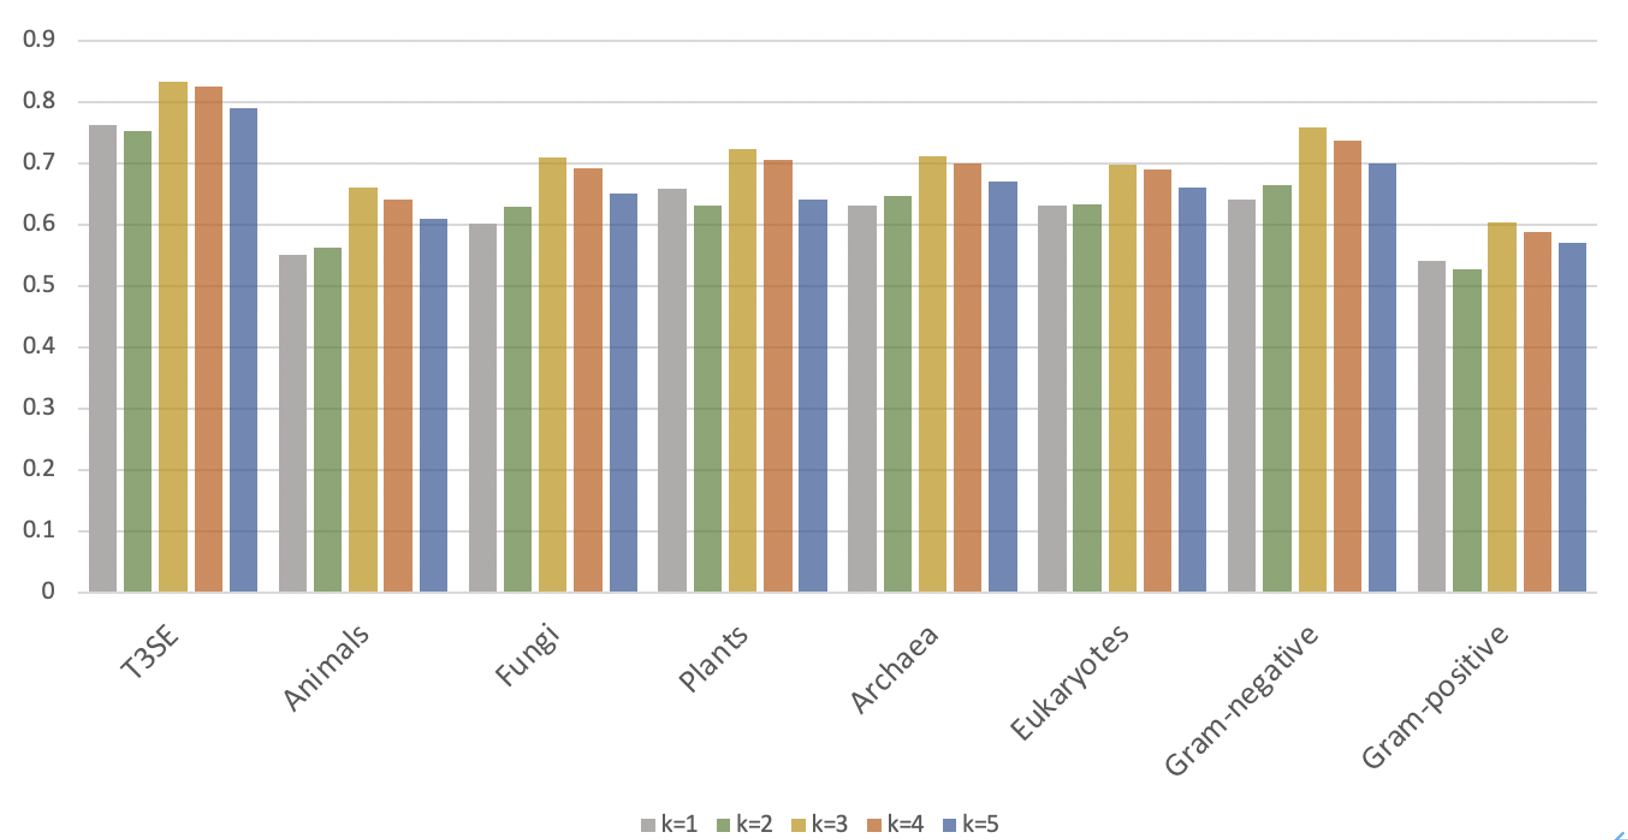
\includegraphics[width=1\textwidth]  {imgs/k-mer.png}
\bicaption[不同 k 值下 ProtPlat 模型的 $F_1$ 值比较]
        {不同 k 值下 ProtPlat 模型的 $F_1$ 值比较。}
        {Comparison of F1 scores obtained by ProtPlat with different values of k.}
\label{fig:k-mer}
\end{figure}


\section{ProtPlat web server}
我们将 ProtPlat 模型作为可供公众访问的网络服务 (https://compbio.sjtu.edu.cn/)。 Web server 的首页界面如图 \ref{fig:web-home} 所示。其中,Home Tab 是 ProtPlat web server的首页介绍,Upload Tab 是上传界面,如图 \ref{fig:web-upload}所示,用户可以按照界面上的要求上传任务的训练集和测试集。Web server upload 的背景模型是经过基于 Pfam 数据库的家族分类任务进行预训练的嵌入表征学习模型,可以用于进行蛋白质分类任务预测。用户可以将自己的训练集和测试集上传到服务器,系统将使用上传的训练集数据对预训练的 Prot Plat 模型进行微调,并在网页上就会显示测试数据集的预测结果。此外,用户还可以下载基于预训练的 ProtPlat 模型氨基酸嵌入向量(在下载选项卡中)。

由于在许多蛋白质分类问题中,训练集太小而无法支持从输入数据中学习好的蛋白质嵌入表征,在许多蛋白质分类问题共享从其氨基酸序列中提取的共同特征,小数据任务可以从两阶段训练策略(预训练 + 微调)中受益很多。


\begin{figure}[!htbp] 
\centering
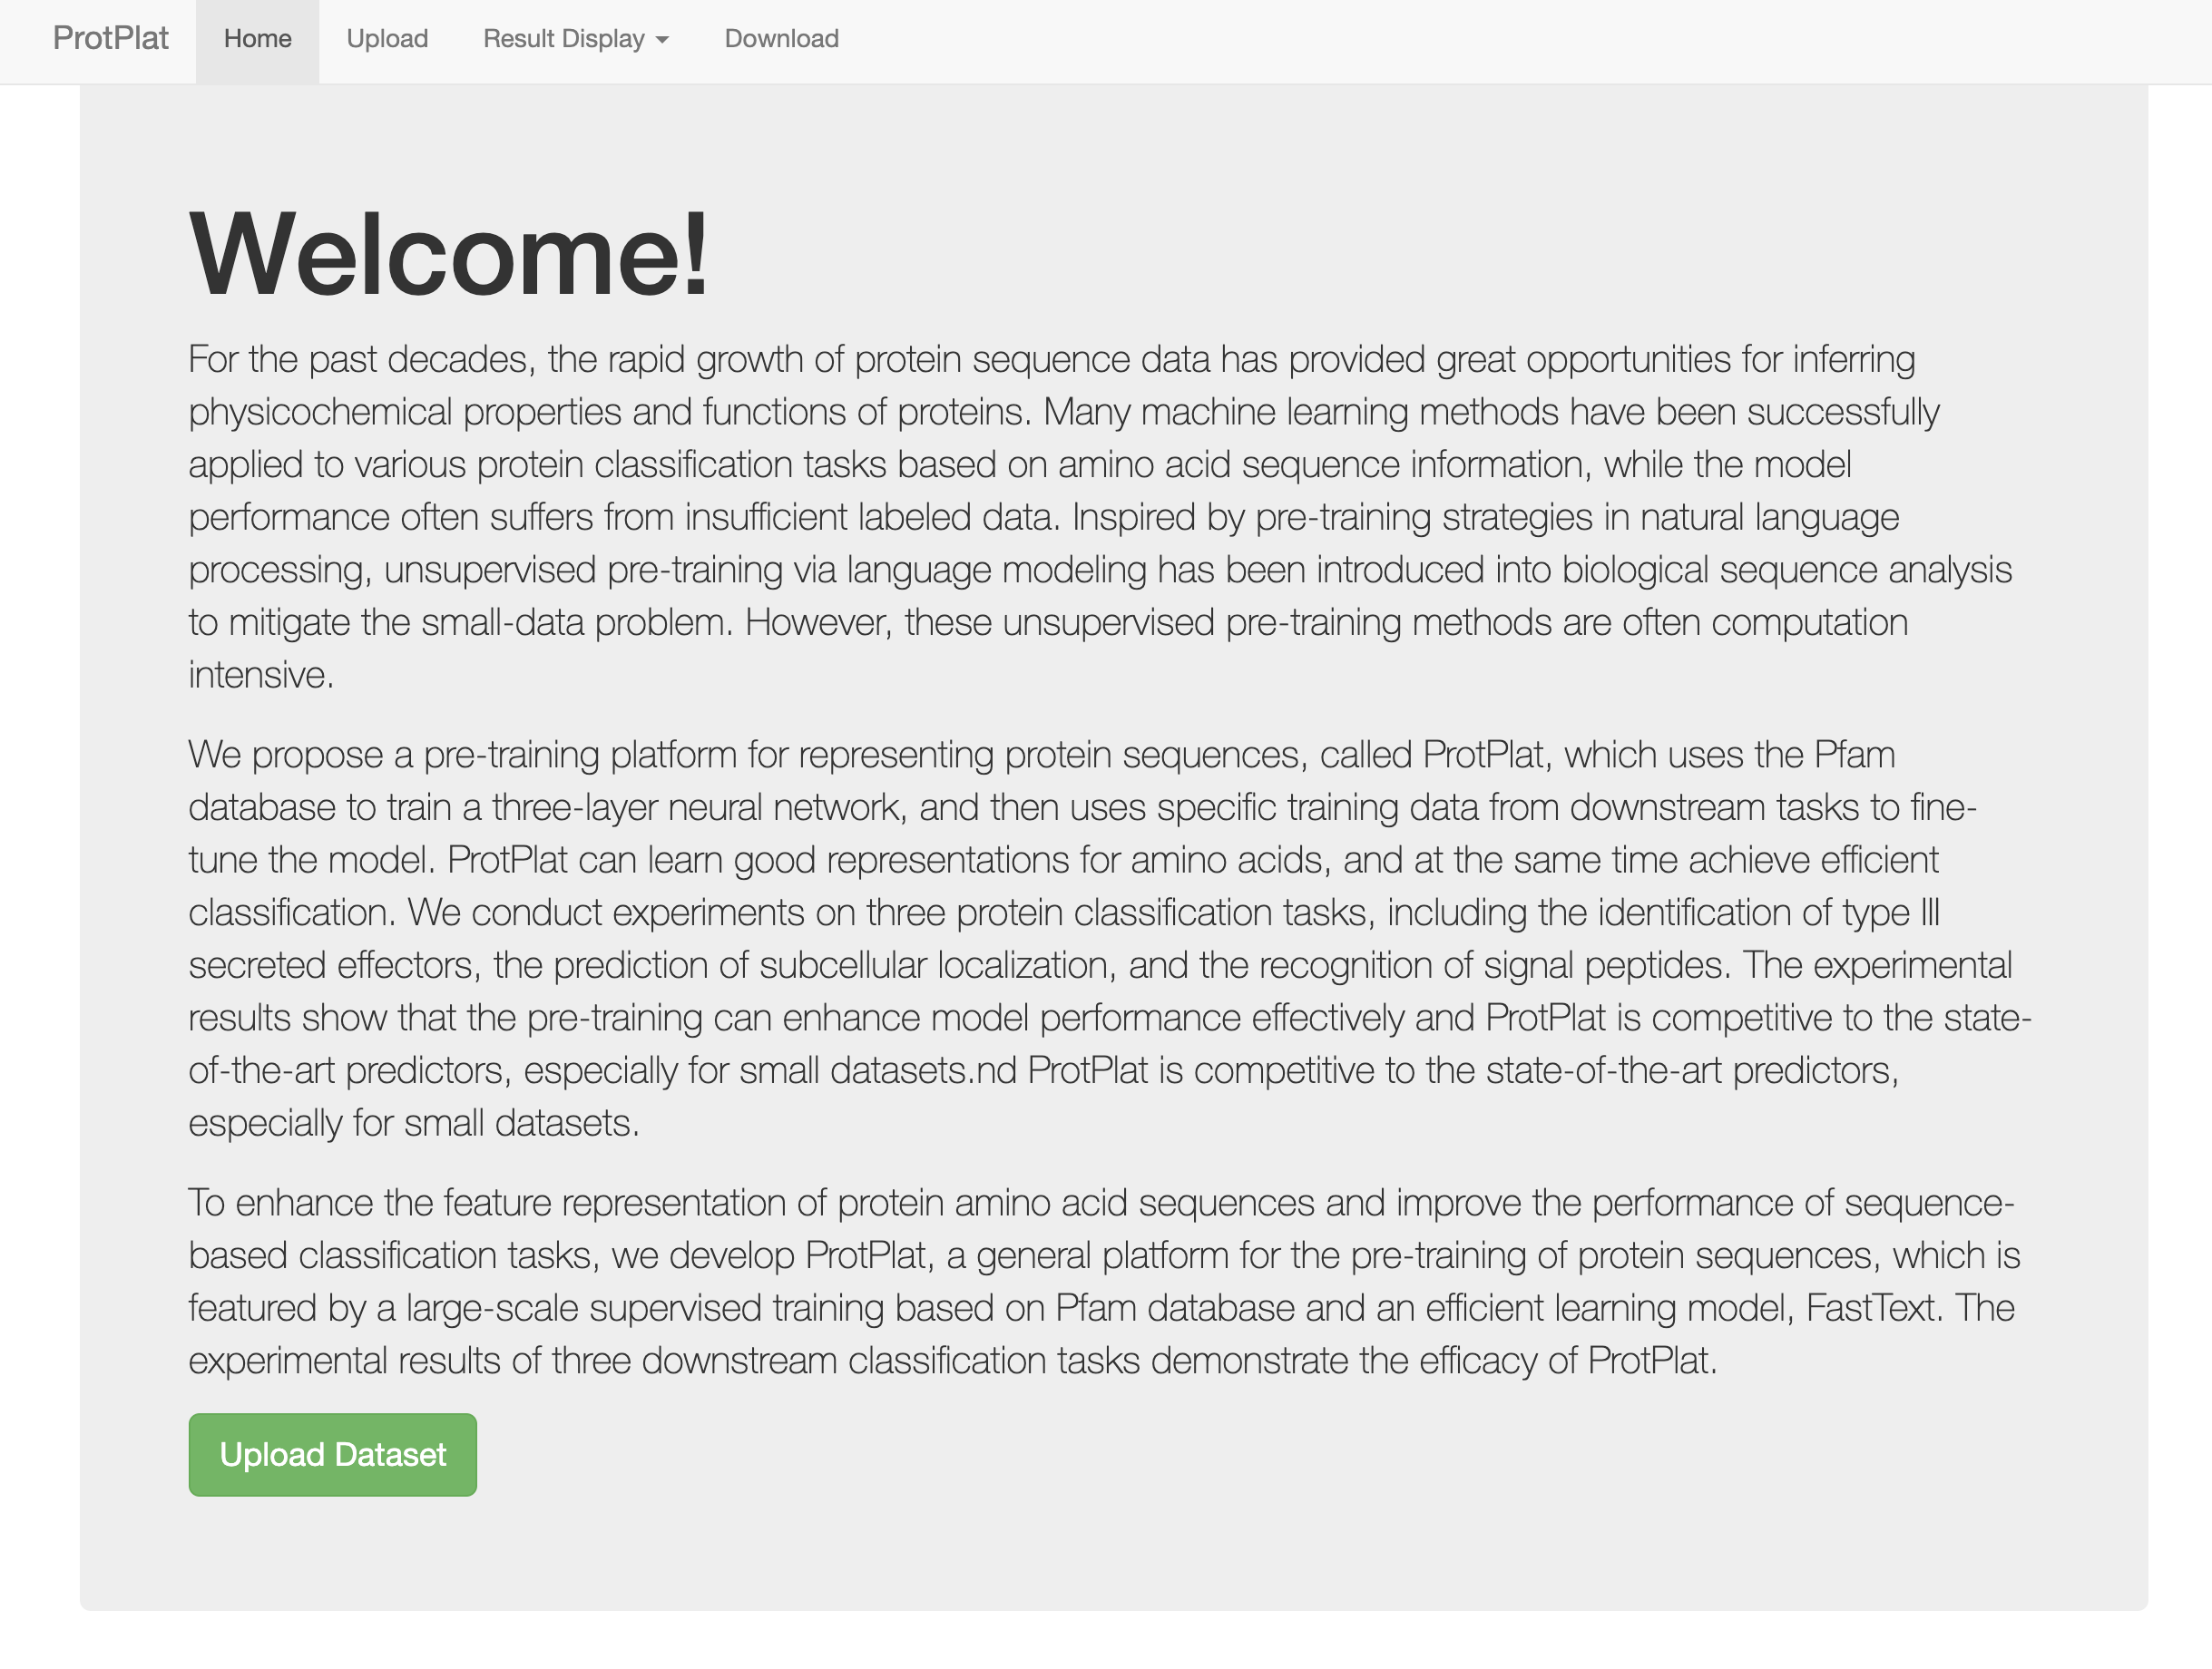
\includegraphics[width=0.8\textwidth]  {imgs/web-home.png}
\bicaption[ProtPlat 的 Web server 首页]
        {ProtPlat 的 Web server 首页。}
        {ProtPlat's web server homepage.}
\label{fig:web-home}
\end{figure}

\begin{figure}[!htp] 
\centering
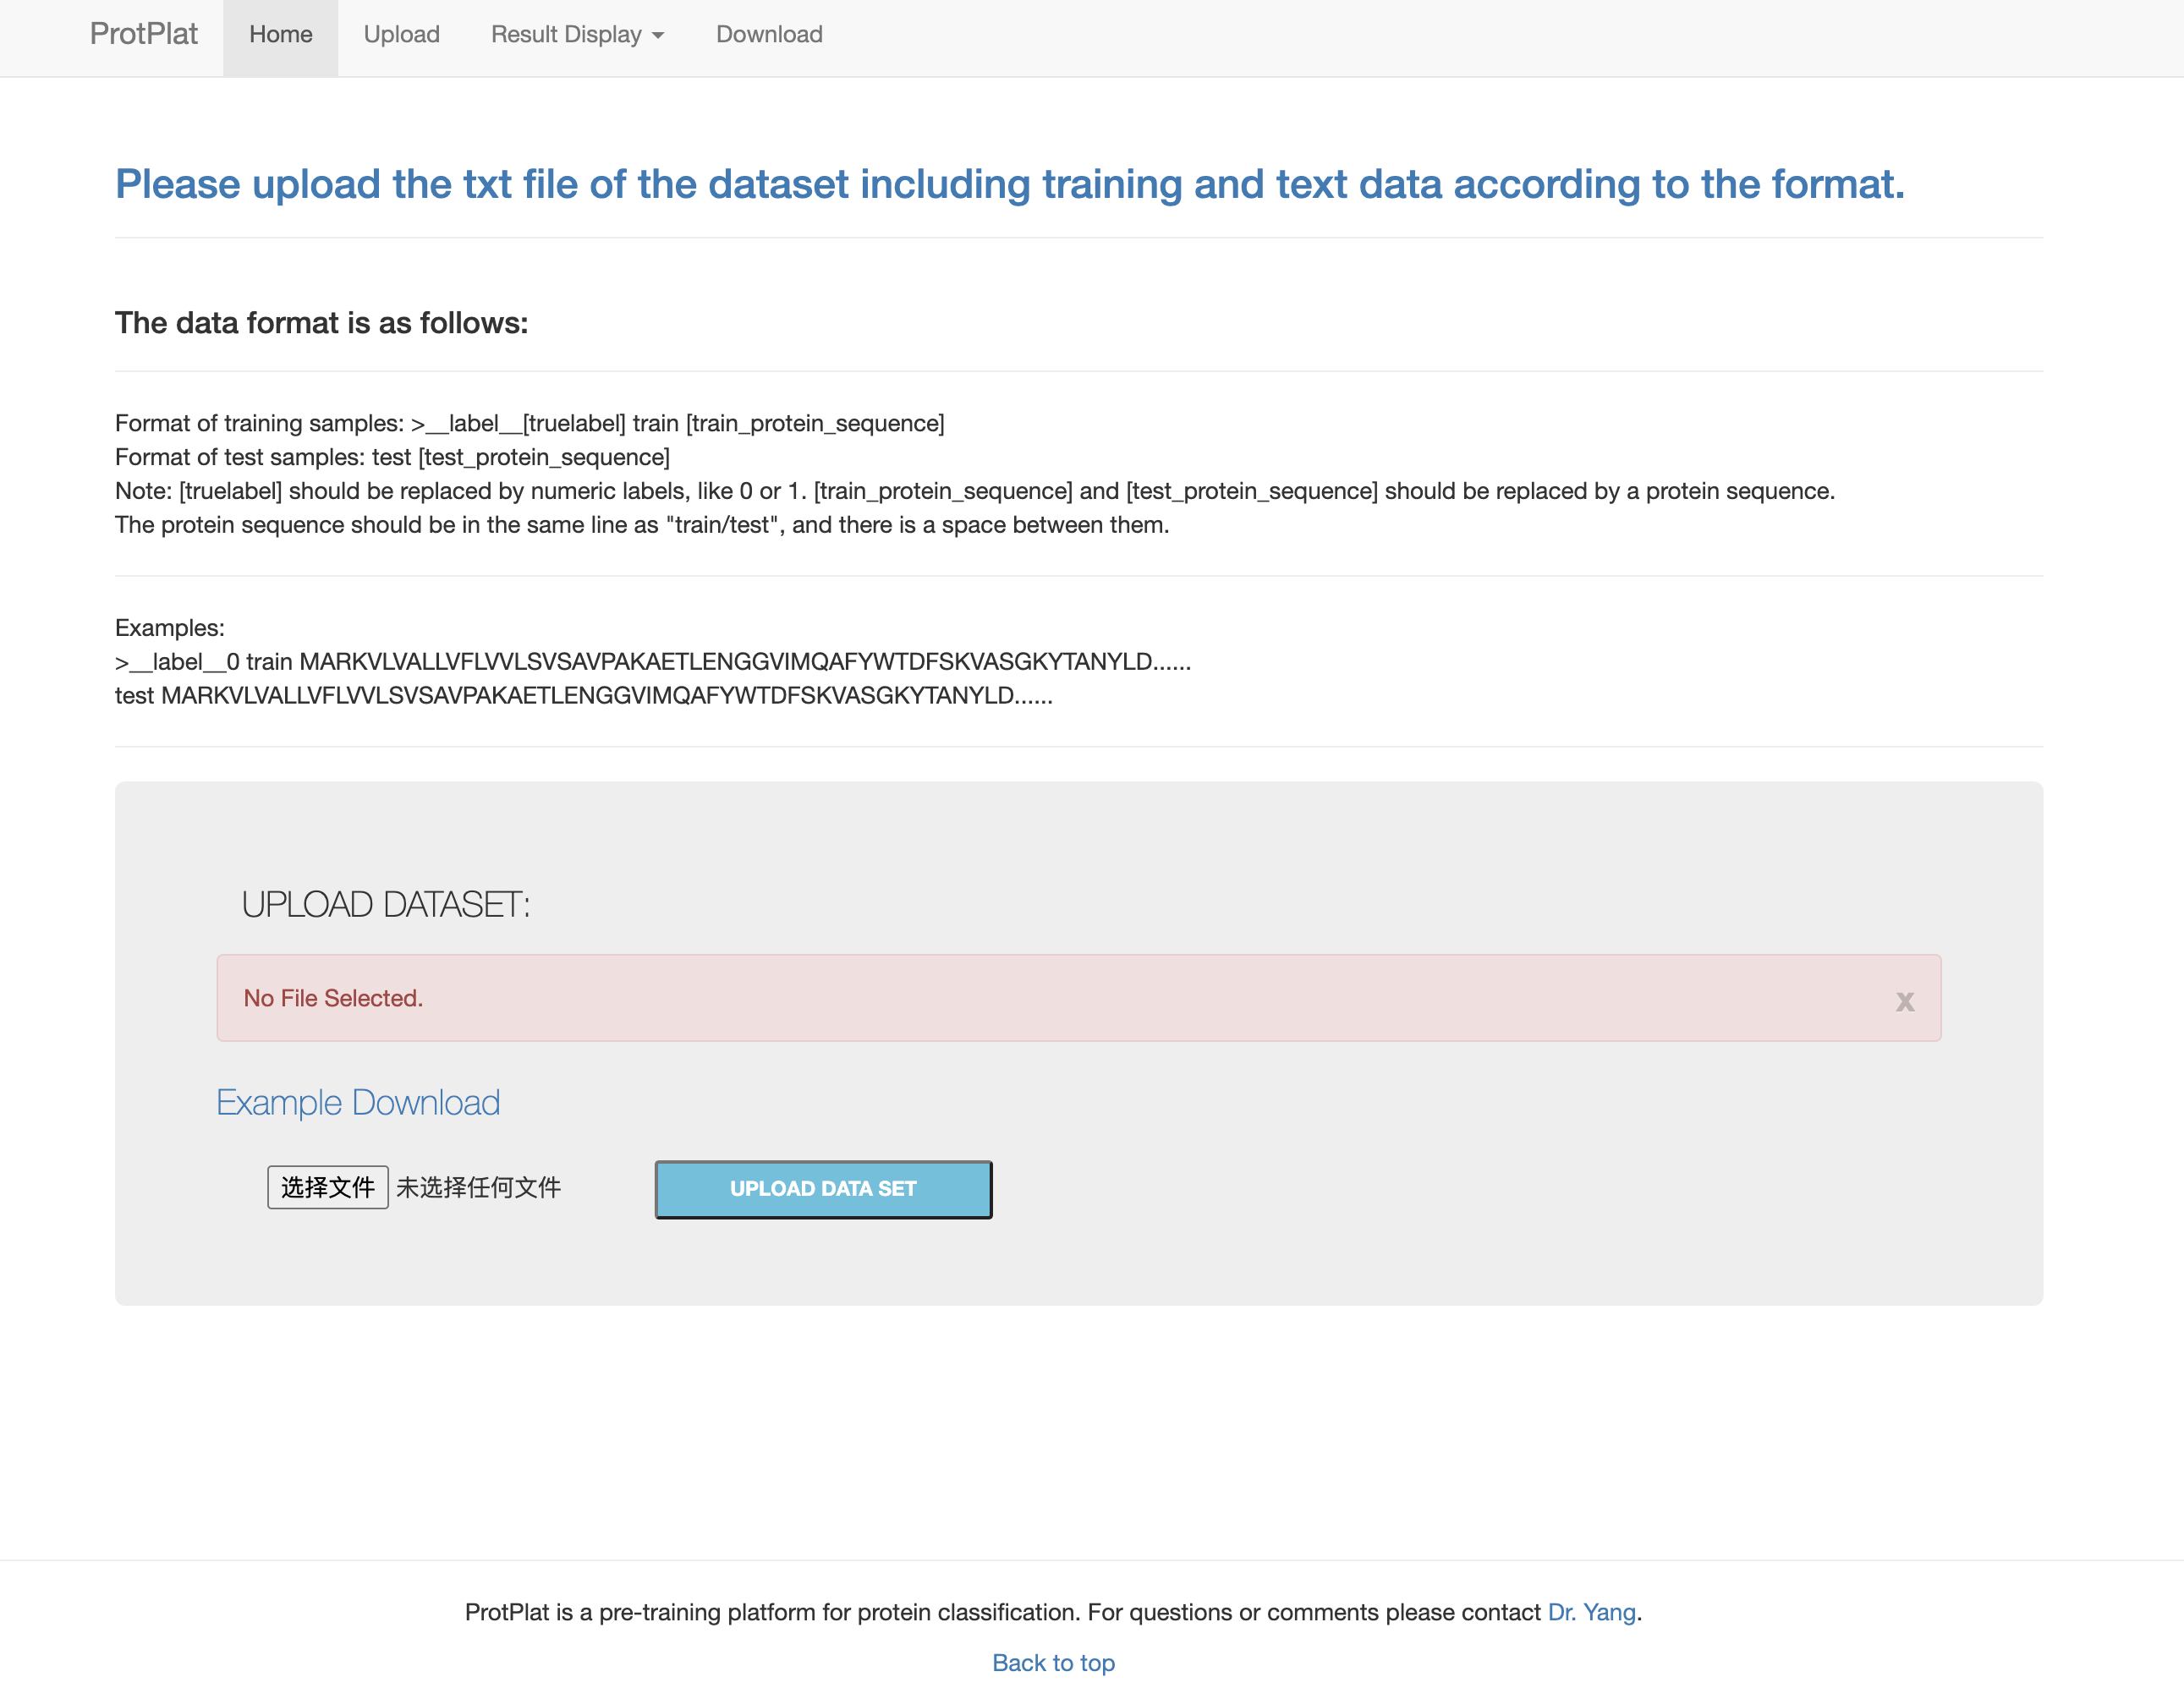
\includegraphics[width=0.8\textwidth]  {imgs/web-upload.png}
\bicaption[ProtPlat 的 Web server 首页]
        {ProtPlat 的 Web server 上传界面。}
        {ProtPlat's web server upload page.}
\label{fig:web-upload}
\end{figure}


\section{本章小结}
本章详细介绍了我们提出的基于有监督预训练得到的 ProtPlat 模型,可以在预训练阶段对大型数据库的蛋白质序列进行嵌入表征学习,在下游任务中对模型进行微调并解决蛋白质序列的分类问题。我们首先介绍了预训练和下游任务所需的实验数据集,接着从数据处理,模型介绍和实验结果三个方面详细介绍了 ProtPlat 模型基于预训练的蛋白质序列嵌入表征学习和基于微调的解决蛋白质序列分类任务两阶段过程。我们在下游的蛋白质序列分类任务中验证了嵌入表征学习具有良好的预测结果,并且通过消融实验验证了蛋白质序列划分的可行性和预训练过程中超参数选取的合理性。
